\section{Architecture}
\begin{description}[style=unboxed]
    \item[How many input neurons are needed for this assignment?]
    There are 10 numerical values for features of the objects, so it's natural to use 10 input neurons.
    \item[How many output neurons do you require?]
    There are 7 possibilities of classes. We could define a value for every one of these classes and use 1 output neuron and train it to output the specific we want for every class. However a more logical choice would be having 7 output neurons, where we associate every output neuron with a specific class. In this way we can train the network to output a 1 on the related output neuron for an object of specific class and 0 on the other 6 neurons.
    \item[How many hidden neurons will your network have?]
    An amount of hidden neurons which is around the same as the amount of input and output neurons is generally accepted as a good practice. So we will start with using 8 hidden neurons.
    \item[Which activation function(s) will you use?]
    We will want our model to be non-linear, because we can't assume anything about the shape of the solution space. So the likely candidate is the logistic function. Another possibility is using tanh, which could be tested if the logistic function is found to not provide a good enough performance.
    \item[Give a schematic diagram of your complete network]
    \end{description}
	
    \tikzset{%
  every neuron/.style={
    circle,
    draw,
    minimum size=0.8cm
  },
  neuron dots/.style={
    draw=none, 
    scale=2,
    text height=0.333cm,
    execute at begin node=\color{black}$\vdots$
  },
}

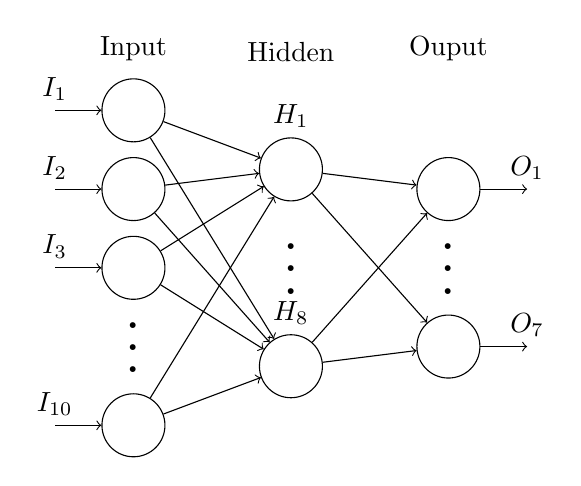
\begin{tikzpicture}
\foreach \m [count=\y] in {1,2,3,dots,4}
  \node [every neuron/.try, neuron \m/.try] (input-\m) at (0,2.5-\y) {};

\foreach \m [count=\y] in {1,dots,2}
  \node [every neuron/.try, neuron \m/.try ] (hidden-\m) at (2,2-\y*1.25) {};

\foreach \m [count=\y] in {1,dots,2}
  \node [every neuron/.try, neuron \m/.try ] (output-\m) at (4,1.5-\y) {};

\foreach \l [count=\i] in {1,2,3,10}
  \draw [<-] (input-\i) -- ++(-1,0)
    node [above] {$I_{\l}$};

\foreach \l [count=\i] in {1,8}
  \node [above] at (hidden-\i.north) {$H_{\l}$};

\foreach \l [count=\i] in {1,7}
  \draw [->] (output-\i) -- ++(1,0)
    node [above] {$O_{\l}$};

\foreach \i in {1,2,3,4}
  \foreach \j in {1,2}
    \draw [->] (input-\i) -- (hidden-\j);

\foreach \i in {1,2}
  \foreach \j in {1,2}
    \draw [->] (hidden-\i) -- (output-\j);

\foreach \l [count=\x from 0] in {Input, Hidden, Ouput}
  \node [align=center, above] at (\x*2,2) {\l};

\end{tikzpicture}

\section{Training}
\begin{description}[style=unboxed]
    \item[How and why did you divide your data into a training, validation and test set?]
    The division into a training, validation and test set is needed because if you just use a training set you'll have no reasonable way to know when to stop training, because using it itself as the validation set will generally give a lower error, so could stop training too quickly. So we will need a validation set for determining the end of the training.\\
    To also gain a measure of the error in classifying new unknown objects we will need another set for which we already know the real class. However if we've already used this set as validation or training set this could again give a falsely high estimate of expected error. For the training set this is obvious, and the validation set will only stop training when the network is decently good at classifying it, so using that as the test set would also give a false impression of how good the network functions, because by definition it'll already have a low error. In choosing the sizes for validation and tests sets we will want to make sure that we still have a large enough training set, while the training and validation sets will need to be large enough that we can expect that a good performance on them will likely also signify a good performance on any general input. For this we chose to use 500 of the known objects as validation data and 500 as testing data.
    \item[How do you evaluate the performance of your network?]
    We examine the summed square errors for the network over the validation set. Another possibility is using the amount of cases in which the actual class of the object in the test set was the highest output in the network, because that's how we will decide our classification after the training. However the sum squared error gives a more general picture of the likelihood of correct classification and so we will use that.
    \item[When and why do you decide to end the training?]
    We will again use the summed squared error as a measure of merit. Through experimental testing we found that the summed squared error normalised over the number of validation cases ceased to decrease at 0,1. So we will use a value slightly higher than that as our cutoff point, which we will take as 0,105.
    \item[Train your network 10 times, each with different initial weights. How does the initialization impact the performance?]
    It doesn't have any significant effect on the minimum sum squared error that is reached, however it does have a small effect on the speed of convergence to this minimum, it could take 3 epochs less. It also had an effect on which objects it classified incorrectly, which immediately makes you think of using multiple networks started with different initialisations and then taking classification that is given most frequently for a given object as it's actual classification. Doing this with the test set showed in increase from on average 450/500 correct to 465/500.
\end{description}

    
    
    
    
    
    
    
    
    
    
    
    
    
    
    
    
    
    
    